\section{Secondary Storage}

\paragraph{Secondary Storage --- Structure}
\begin{itemize}
  \item hard disk drives
  \item solid state drive
  \item RAID structure
  \item tertiary storage devices (DVD, magnetic tape)
\end{itemize}

\paragraph{Hard Disk Drives --- Anatomy}
\begin{itemize}
  \item stack of magnetic platters
  \item disk arms contain disk heads per recording surface, read/write to platters
  \item \textbf{Storage}:
  \begin{itemize}
    \item platters divided into concentric \emph{tracks}
    \item \emph{cylinder}: stack of tracks of fixed radius
    \item tracks of fixed radius divided into \emph{sectors}
  \end{itemize}
\end{itemize}

\paragraph{Flash Memory}
\begin{itemize}
  \item \textbf{advantages}:
  \begin{itemize}
    \item[+] solid state
    \item[+] lower power consumption/heat
    \item[+] no mechanical seek 
  \end{itemize}
  \item \textbf{disadvantages}:
  \begin{itemize}
    \item[-] limited number of overwrites
    \item[-] limited durability 
  \end{itemize}
\end{itemize}

\paragraph{RAID}
\begin{itemize}
  \item \textbf{Idea}: improve performance/reliability of storage system by storing redundant data
\end{itemize}
\begin{figure}[h]\centering\label{RAID}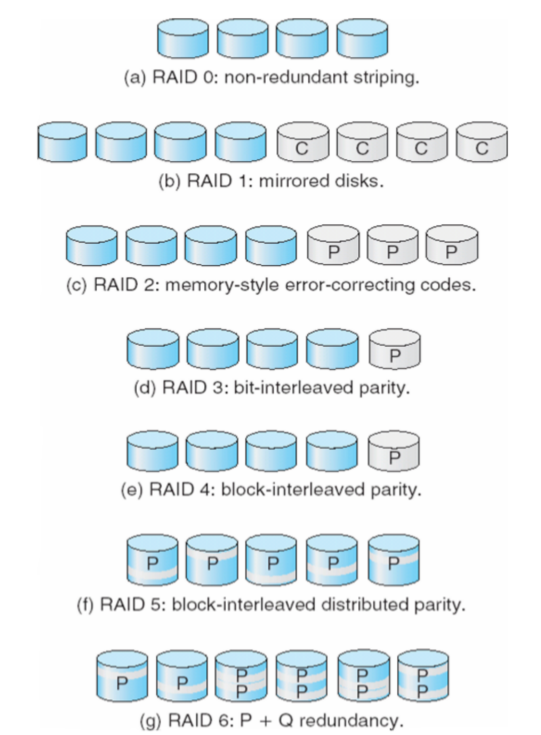
\includegraphics[width=0.2\textwidth]{RAID}\end{figure}